\documentclass{exam}
\usepackage{../../commonheader}
\usepackage{graphicx}
\usepackage{color}

%%% CHANGE THESE %%%%%%%%%%%%%%%%%%%%%%%%%%%%%%%%%%%%%%%%%%%%%%%%%%%%%%%%%%%%%%
\discnumber{}
\title{\textsc{Midterm 2 Review}}
\date{March 12, 2017}
%%%%%%%%%%%%%%%%%%%%%%%%%%%%%%%%%%%%%%%%%%%%%%%%%%%%%%%%%%%%%%%%%%%%%%%%%%%%%%%

\begin{document}
\maketitle
\rule{\textwidth}{0.15em}
\fontsize{12}{15}\selectfont

%%% INCLUDE TOPICS HERE %%%%%%%%%%%%%%%%%%%%%%%%%%%%%%%%%%%%%%%%%%%%%%%%%%%%%%%


%%% Question %%%

\section{List Mutation}
\begin{questions}

\item Draw the Box and Pointer!
\newline
\begin{lstlisting}
>>> corgi = [3, 15, 18, 7, 9]
>>> husky = [8, 21, 19, 11, 25]
>>> poodle = corgi.pop()
>>> corgi += husky[-3:]
\end{lstlisting}
\begin{solution}
\begin{lstlisting}

\end{lstlisting}
\end{solution}
\vspace{4cm}

\item Draw the Box and Pointer!

\begin{lstlisting}
>>> pom = [16, 15, 13]
>>> pompom = pom * 2
>>> pompom.append(pom[:])
>>> pom.extend(pompom)
\end{lstlisting}

\end{questions}
\clearpage

\section{OOP}
\begin{questions}
\item The fOOd Chain
\begin{lstlisting}
class Animal:
    kingdom = []
    location = 'Earth'
    def __init__(self, type, prey):
        self.type = type
        self.prey = prey
        self.kingdom.append(self)
        self.food_chain = [self]
    def eat(self):
        self.location = 'Mars'
    def __repr__(self):
        return self.type
    
class Predator(Animal):
    def eat(self):
        for animal in self.kingdom:
            if repr(animal) == self.prey:
                self.food_chain.extend(animal.food_chain)
                self.kingdom.remove(animal)
    def __str__(self):
        return '{}s eat {}s.'.format(self.type, self.prey)

grasshopper = Animal('Grasshopper', 'Grass')
sparrow = Predator('Sparrow', 'Grasshopper')
hawk = Predator('Hawk', 'Sparrow')
\end{lstlisting}
\clearpage
For each of the expressions in the table below, write the output displayed by the interactive Python interpreter when the expression is evaluated. The output may have multiple lines. If more than 3 lines are displayed, just write the first 3. If an error occurs, write “Error”. If evaulation would run forever, write “Forever”.\\
Assume that you have started \texttt{python3} and executed the following statements:

\begin{center}
\begin{tabular}{ |p{8cm}|p{6cm}| } 
 \hline
 \begin{lstlisting}
>>> sparrow.kingdom 
\end{lstlisting} &  \\  \hline
 \begin{lstlisting}
>>> print(grasshopper)
\end{lstlisting} &  \\  \hline
 \begin{lstlisting}
>>> Animal.eat(grasshopper)
>>> grasshopper.location
\end{lstlisting} &  \\  \hline
 \begin{lstlisting}
>>> hawk.location
\end{lstlisting} &  \\  \hline
 \begin{lstlisting}
>>> print(hawk)
\end{lstlisting} &  \\  \hline
 \begin{lstlisting}
>>> sparrow.eat()
>>> sparrow.food_chain
\end{lstlisting} &  \\  \hline
 \begin{lstlisting}
>>> hawk.eat()
>>> hawk.location
\end{lstlisting} &  \\  \hline
 \begin{lstlisting}
>>> hawk.kingdom
\end{lstlisting} &  \\  \hline
 \begin{lstlisting}
>>> hawk.food_chain
\end{lstlisting} &  \\  \hline
 \begin{lstlisting}
>>> grasshopper.food_chain
\end{lstlisting} &  \\  \hline
\end{tabular}
\end{center}

\clearpage

\item The fOOd Chain
\begin{lstlisting}
class Bird:
    def __init__(self, call):
        self.call = call
        self.can_fly = True
    def fly(self):
        if self.can_fly:
            return 'Don't stop me now!'
        else:
            return 'Ground control to Major Tom...'
    def speak(self):
        print(self.call)  
\end{lstlisting}
\begin{lstlisting}
class Chicken(Bird):
    def speak(self, other):
        super().speak()
        other.speak()

class Penguin(Bird):
    can_fly = False
    def speak(self):
        call = 'Ice to meet you'
        print(call)

andre = Chicken('cluck')
gunter = Penguin('noot')
\end{lstlisting}
\clearpage
For each of the expressions in the table below, write the output displayed by the interactive Python interpreter when the expression is evaluated. The output may have multiple lines. If more than 3 lines are displayed, just write the first 3. If an error occurs, write “Error”. If evaulation would run forever, write “Forever”.\\
Assume that you have started \texttt{python3} and executed the following statements.

\begin{center}
\begin{tabular}{ |p{8cm}|p{6cm}| } 
 \hline
 \begin{lstlisting}
>>> andre.speak(Bird('coo'))
\end{lstlisting} &  \\  \hline
 \begin{lstlisting}
>>> andre.speak()
\end{lstlisting} &  \\  \hline
 \begin{lstlisting}
>>> gunter.fly()
\end{lstlisting} &  \\  \hline
 \begin{lstlisting}
>>> andre.speak(gunter)
\end{lstlisting} &  \\  \hline
 \begin{lstlisting}
>>> Bird.speak(gunter)
\end{lstlisting} &  \\  \hline
\end{tabular}
\end{center}
\end{questions}
\clearpage

\section{Linked Lists and Trees}
\begin{questions}
\item For each of the following code fragments, add arrows and values to the object skeletons to the right to show the final state of the program. Single boxes are variables that contain pointers. Double boxes are Links. Not all boxes need be used.\\
\begin{center}
\vspace{1cm}
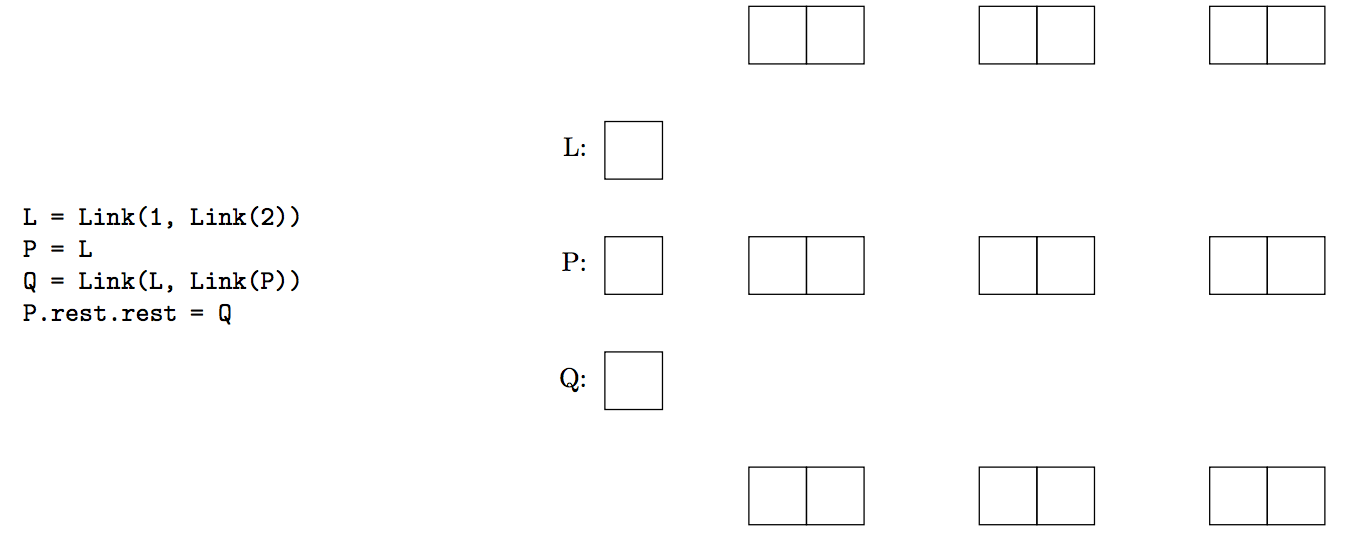
\includegraphics[width=15cm]{a}\\
\vspace{5cm}
 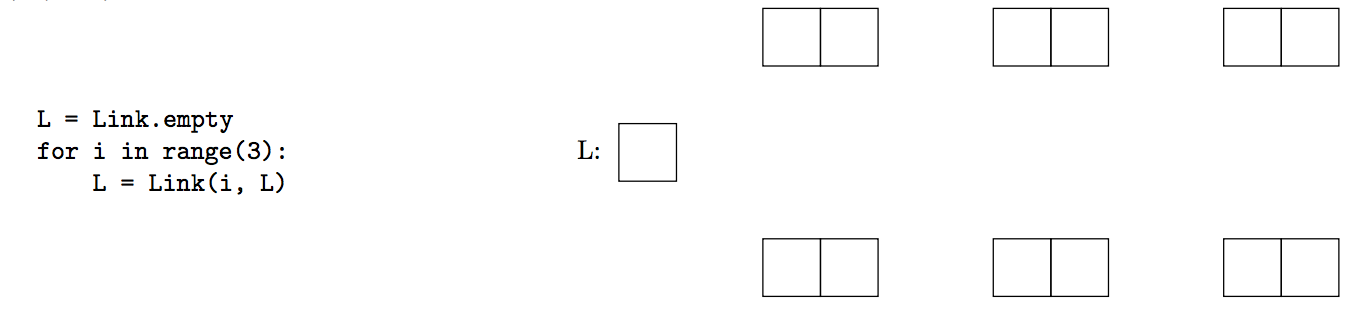
\includegraphics[width=15cm]{b}
\end{center}

\clearpage

\item WWPD? Try drawing a box-and-pointer diagram!
\begin{lstlisting}
def wild(lnk):
    if lnk is Link.empty or lnk.rest is Link.empty:
        return lnk
    breath = wild(lnk.rest)
    lnk.rest.rest = lnk
    lnk.rest = NULL
    return breath
\end{lstlisting}

\begin{center}
\begin{tabular}{ |p{8cm}|p{6cm}| } 
 \hline
 \begin{lstlisting}
>>> triforce = Link(3, Link(1, Link(4)))
>>> wild(triforce)
\end{lstlisting} &  \\  \hline
 \begin{lstlisting}
>>> triforce
\end{lstlisting} &  \\  \hline
\end{tabular}
\end{center}

\item The depth of a node from the root of a tree is measured by its distance from the root. Nodes that have the same depth are said to be on the same 'level'. 
Write a function that returns a dictionary, where each key is a level and each value is a list of all labels on that level. 
 \begin{lstlisting}
def one_more_level(t):

    level_dict = _________________
    
    def traverse(t, level):
    
        if level in queue:
        
            queue[level] = _________________
            
        else:
        
            queue[level] = _________________
            
        for _________________:
        
            traverse(_________________, _________________)
            
    traverse(________________, ______________________)
    
    return _________________
\end{lstlisting}

\end{questions}

\section{Iterators/Generators}
\begin{questions}
\item Write an iterator that takes a Linked List and iterates through it. For instance: 
\begin{lstlisting}
>>> li = ListIterator(Link(1, Link(2, Link(3))))
>>> next(li)
1
>>> next(li)
2
>>> next(li)
3
>>> next(li)
StopIteration

class LinkIterator:
\end{lstlisting}
\vspace{3cm}

\item Write a generator that outputs the a decoded run length sequence.
\begin{lstlisting}
def run_length_decoder(encoding):
   """
   >>> rld = run_length_decoder([("h", 1), ("e", 1), ("l", 2), ("o", 1)])
   >>> lst(rld)
   ["h", "e", "l", "l", "o"]
   """
   
\end{lstlisting}
\end{questions}
\vspace{3cm}


\section{Orders of Growth}
\begin{questions}
\item What do these runtimes simplify to? \newline
\begin{tabular}{ |p{2cm}|p{2cm}|p{4cm}|p{4cm}| } 
\hline 
O($30n$)& O($10000$) & O($n^2 + 10n + 1$) & O($100 + 2^n + n^50$) \\ \hline
 & & & \\
\hline 
\end{tabular}

\item What is the runtime?

\begin{center}
\begin{tabular}{ |p{13cm}|p{2cm}| } 
 \hline
 \begin{lstlisting}
def m(n):
    if n % 7 == 0:
        return m (n - 1) + m(n - 2) * m (n -3)
    else:
        return n
\end{lstlisting} &  \\  \hline
 \begin{lstlisting}
def rec(n):
    if n == 1:
        return 1
    return rec(n - 1)
\end{lstlisting} &  \\  \hline
 \begin{lstlisting}
def rec(n):
    if n == 1:
        return 1
    return rec(n - 1) + rec(n - 1)
\end{lstlisting} &  \\  \hline
 \begin{lstlisting}
def rec(n):
    if n == 1:
        return 1
    return rec(n//2)
\end{lstlisting} &  \\  \hline
 \begin{lstlisting}
def wow(n): 
    if n == 1:
        return 1
    while n != 0: 
        if n % 2 == 1: 
            return wow(n // 2) + 1
        n -= 1
\end{lstlisting} &  \\  \hline
 \begin{lstlisting}
def pow(n):
    for x in range(50 * n):
        print("powwow")
    for x in range(n ** 2):
        wow(n ** 2)
\end{lstlisting} &  \\  \hline
\end{tabular}
\end{center}

\clearpage

\item Find the runtime in terms of m and n, where m is the \texttt{len(lst1)} and \texttt{n} is the \texttt{len(lst2)}
Assume append and * are constant time operations
\begin{lstlisting}
def createMatrix(lst1, lst2): 
    """
    >>> createMatrix([1, 2], [3, 4, 5])
    [[3, 4, 5], [6, 8, 10]]
    """ 
    matrix = []
    for elem in lst1:
        row = []
        For elem in lst2:
            row.append(lst1 * lst2)
            matrix.append(row)
        return matrix
\end{lstlisting}
Circle one of the options below:
\begin{itemize}
\item O($n + m$)
\item O($m$)
\item O($n^2 + m^2$)
\item O($n * m$)
\end{itemize}

\item Runtime with Linked Lists\\
Let $n$ be the number of elements IN a linked list.\\
Let $m$ be the number of elements ADDED to the linked list.
\begin{enumerate}
\item What is the runtime of adding 1 link to the beginning of a linked list?
\vspace{1cm}
\item What is the runtime of adding 1 link to the end of a linked list?
\vspace{1cm}
\item What is the runtime of adding m links to the beginning of a linked list?
\vspace{1cm}
\item What is the runtime of adding m links to the end of empty linked list?
\end{enumerate}

\end{questions}


%%%%%%%%%%%%%%%%%%%%%%%%%%%%%%%%%%%%%%%%%%%%%%%%%%%%%%%%%%%%%%%%%%%%%%%%%%%%%%%

\end{document}
